\textbf{Explica brevemente qué es un agente racional en el contexto de inteligencia artificial. Preferiblemente incluye un diagrama en tu descripción (1 pt.).}\vspace{.3cm}

Un agente racional es una entidad que busca maximizar su función de utilidad; existe en un entorno y es capaz de percibirlo con sus sensores y, posteriormente, actúa sobre él mediante sus actuadores. De manera simple, un agente racional es una entidad que realiza las acciones que más sentido tienen para cumplir sus objetivos. \vspace{.3cm}

Para ilustrarlo de manera más gráfica, se incluye un diagrama creado por ICCSI: \vspace{.3cm}

\begin{figure}[H]
    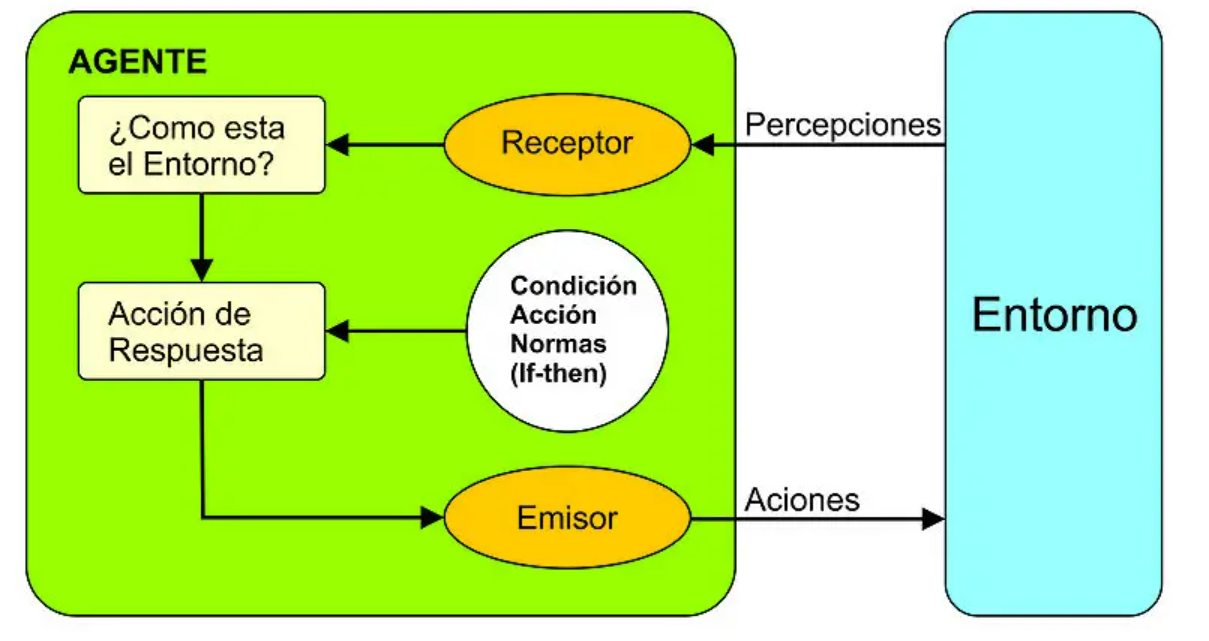
\includegraphics[width=10cm]{src/Img/que-es-un-agente-software-racional-1.png}
    \centering
    \caption{\cite{iccsi_agente_racional_imagen}}
\end{figure}

Como podemos ver, la definición de agente es lo suficientemente amplia para ser utilizada en diversos contextos.

\cite{russell2020artificial}
